\documentclass[12pt]{article}
\usepackage[utf8]{inputenc}
\usepackage[utf8]{inputenc}
\usepackage{amsmath}
\usepackage{amsthm}
\usepackage{amssymb}
\usepackage{array}
\usepackage{geometry}
\usepackage{amsfonts}
\usepackage{mathrsfs}
\usepackage{bm}
\usepackage{hyperref}
\usepackage{float}
\usepackage[dvipsnames]{xcolor}
\usepackage[inline]{enumitem}
\usepackage{mathtools}
\usepackage{changepage}
\usepackage{graphicx}
\usepackage{systeme}
\usepackage{caption}
\usepackage{subcaption}
\usepackage{tcolorbox}
\usepackage[linguistics]{forest}
\usepackage{tikz}
\usetikzlibrary{matrix, patterns, decorations.pathreplacing, calligraphy}
\usepackage{tikz-cd}
\usepackage[nameinlink]{cleveref}
\geometry{
headheight=15pt,
left=60pt,
right=60pt
}
\setlength{\emergencystretch}{20pt}
\usepackage{fancyhdr}
\pagestyle{fancy}
\fancyhf{}
\lhead{}
\chead{Section 8.2 Exercises}
\rhead{\thepage}
\hypersetup{
    colorlinks=true,
    linkcolor=blue,
    urlcolor=blue
}

\theoremstyle{definition}
\newtheorem*{remark}{Remark}

\newtheoremstyle{exercise}
    {}
    {}
    {}
    {}
    {\bfseries}
    {.}
    { }
    {\thmname{#1}\thmnumber{#2}\thmnote{ (#3)}}
\theoremstyle{exercise}
\newtheorem{exercise}{Exercise 8.2.}

\newtheoremstyle{solution}
    {}
    {}
    {}
    {}
    {\itshape\color{magenta}}
    {.}
    { }
    {\thmname{#1}\thmnote{ #3}}
\theoremstyle{solution}
\newtheorem*{solution}{Solution}

\Crefformat{exercise}{#2Exercise 8.2.#1#3}

\tcbset{colback=blue!5!white}

\newcommand{\interior}[1]{%
  {\kern0pt#1}^{\mathrm{o}}%
}
\newcommand{\ts}{\textsuperscript}
\newcommand{\setcomp}[1]{#1^{\mathsf{c}}}
\newcommand{\poly}{\mathcal{P}}
\newcommand{\quand}{\quad \text{and} \quad}
\newcommand{\quimplies}{\quad \implies \quad}
\newcommand{\quiff}{\quad \iff \quad}
\newcommand{\N}{\mathbf{N}}
\newcommand{\Z}{\mathbf{Z}}
\newcommand{\Q}{\mathbf{Q}}
\newcommand{\I}{\mathbf{I}}
\newcommand{\R}{\mathbf{R}}
\newcommand{\C}{\mathbf{C}}

\DeclarePairedDelimiter\abs{\lvert}{\rvert}
% Swap the definition of \abs* and \norm*, so that \abs
% and \norm resizes the size of the brackets, and the 
% starred version does not.
\makeatletter
\let\oldabs\abs
\def\abs{\@ifstar{\oldabs}{\oldabs*}}

\DeclarePairedDelimiter\norm{\lVert}{\rVert}
\makeatletter
\let\oldnorm\norm
\def\norm{\@ifstar{\oldnorm}{\oldnorm*}}
\makeatother

\DeclarePairedDelimiter\paren{(}{)}
\makeatletter
\let\oldparen\paren
\def\paren{\@ifstar{\oldparen}{\oldparen*}}
\makeatother

\DeclarePairedDelimiter\bkt{[}{]}
\makeatletter
\let\oldbkt\bkt
\def\bkt{\@ifstar{\oldbkt}{\oldbkt*}}
\makeatother

\DeclarePairedDelimiter\set{\{}{\}}
\makeatletter
\let\oldset\set
\def\set{\@ifstar{\oldset}{\oldset*}}
\makeatother

\setlist[enumerate,1]{label={(\alph*)}}

\begin{document}

\section{Section 8.2 Exercises}

Exercises with solutions from Section 8.2 of \hyperlink{ua}{[UA]}.

\begin{exercise}
\label{ex:1}
    Decide which of the following are metrics on \( X = \R^2 \). For each, we let \( x = (x_1, x_2) \) and \( y = (y_1, y_2) \) be points in the plane.
    \begin{enumerate}
        \item \( d(x, y) = \sqrt{ (x_1 - y_1)^2 + (x_2 - y_2)^2 } \).

        \item \( d(x, y) = \max \{ \abs{x_1 - y_1}, \abs{x_2 - y_2} \} \).

        \item \( d(x, y) = \abs{x_1 x_2 + y_1 y_2} \).
    \end{enumerate}
\end{exercise}

\begin{solution}
    \begin{enumerate}
        \item This is a metric on \( \R^2 \). To see this, we shall verify each property in Definition 8.2.1. Let \( x = (x_1, x_2), y = (y_1, y_2) \in \R^2 \) be given.
        \begin{enumerate}[label=(\roman*)]
            \item It is clear that \( d(x, y) \geq 0 \). Observe that
            \begin{align*}
                d(x, y) = 0 &\iff \sqrt{ (x_1 - y_1)^2 + (x_2 - y_2)^2 } = 0 \\[2mm]
                &\iff (x_1 - y_1)^2 + (x_2 - y_2)^2 = 0 \\[2mm]
                &\iff (x_1 - y_1)^2 = 0 \text{ and } (x_2 - y_2)^2 = 0 \\[2mm]
                &\iff x_1 = y_1 \text{ and } x_2 = y_2 \\[2mm]
                &\iff x = y.
            \end{align*}

            \item We have
            \[
                d(x, y) = \sqrt{ (x_1 - y_1)^2 + (x_2 - y_2)^2 } = \sqrt{ (y_1 - x_1)^2 + (y_2 - x_2)^2 } = d(y, x).
            \]

            \item For \( a = (a_1, a_2), b = (b_1, b_2) \in \R^2 \), observe that
            \begin{multline*}
                \sqrt{ (a_1 + b_1)^2 + (a_2 + b_2)^2 } \leq \sqrt{ a_1^2 + a_2^2 } + \sqrt{ b_1^2 + b_2^2 } \\[2mm]
                \iff (a_1 + b_1)^2 + (a_2 + b_2)^2 \leq a_1^2 + a_2^2 + b_1^2 + b_2^2 + 2 \sqrt{ a_1^2 + a_2^2 } \sqrt{ b_1^2 + b_2^2 } \\[2mm]
                \iff a_1 b_1 + a_2 b_2 \leq \sqrt{ a_1^2 + a_2^2 } \sqrt{ b_1^2 + b_2^2 }.
            \end{multline*}
            This last inequality follows from the \href{https://en.wikipedia.org/wiki/Cauchy%E2%80%93Schwarz_inequality#R2_-_The_plane}{Cauchy-Schwarz inequality}. The desired triangle inequality for \( d \) can now be obtained by taking \( a = x - z \) and \( b = z - y \).
        \end{enumerate}

        \item This is a metric on \( \R^2 \). To see this, we shall verify each property in Definition 8.2.1. Let \( x = (x_1, x_2), y = (y_1, y_2) \in \R^2 \) be given.
        \begin{enumerate}[label=(\roman*)]
            \item It is clear that \( d(x, y) \geq 0 \). Observe that
            \begin{align*}
                d(x, y) = 0 &\iff \max \{ \abs{x_1 - y_1}, \abs{x_2 - y_2} \} = 0 \\[2mm]
                &\iff \abs{x_1 - y_1} = 0 \text{ and } \abs{x_2 - y_2} = 0 \\[2mm]
                &\iff x_1 = y_1 \text{ and } x_2 = y_2 \\[2mm]
                &\iff x = y.
            \end{align*}

            \item We have
            \[
                d(x, y) = \max \{ \abs{x_1 - y_1}, \abs{x_2 - y_2} \} = \max \{ \abs{y_1 - x_1}, \abs{y_2 - x_2} \} = d(y, x).
            \]

            \item Let \( z = (z_1, z_2) \in \R^2 \) be given. Suppose that \( d(x, y) = \abs{x_1 - y_1} \) (the case where \( d(x, y) = \abs{x_2 - y_2} \) is handled similarly) and observe that
            \[
                d(x, y) = \abs{x_1 - y_1} \leq \abs{x_1 - z_1} + \abs{z_1 - y_1} \leq d(x, z) + d(z, y).
            \]
        \end{enumerate}

        \item This is not a metric on \( \R^2 \). To see this, observe that by taking \( x = (1, 1) \) and \( y = (-1, 1) \) we obtain \( d(x, y) = 0 \), but \( x \neq y \). Thus property (i) of Definition 8.2.1 is not satisfied.
    \end{enumerate}
\end{solution}

\begin{exercise}
\label{ex:2}
    Let \( C[0, 1] \) be the collection of continuous functions on the closed interval \( [0, 1] \). Decide which of the following are metrics on \( C[0, 1] \).
    \begin{enumerate}
        \item \( d(f, g) = \sup \{ \abs{f(x) - g(x)} : x \in [0, 1] \} \).

        \item \( d(f, g) = \abs{f(1) - g(1)} \).

        \item \( d(f, g) = \int_0^1 \abs{f - g} \).
    \end{enumerate}
\end{exercise}

\begin{solution}
    \begin{enumerate}
        \item This is a metric on \( C[0, 1] \). Note that by the Extreme Value Theorem (Theorem 4.4.2), the supremum is actually a maximum.
        \begin{enumerate}[label=(\roman*)]
            \item Because each element of \( \{ \abs{f(x) - g(x)} : x \in [0, 1] \} \) is non-negative, we must have \( d(f, g) \geq 0 \). Observe that
            \begin{align*}
                d(f, g) = 0 &\iff \max \{ \abs{f(x) - g(x)} : x \in [0, 1] \} = 0 \\[2mm]
                &\iff \abs{f(x) - g(x)} = 0 \text{ for all } x \in [0, 1] \\[2mm]
                &\iff f(x) = g(x) \text{ for all } x \in [0, 1] \\[2mm]
                &\iff f = g.
            \end{align*}

            \item As \( \abs{f(x) - g(x)} = \abs{g(x) - f(x)} \) for each \( x \in [0, 1] \), we see that \( d(f, g) = d(g, f) \).

            \item Let \( h \in C[0, 1] \) be given and suppose that \( \abs{f - g} \) attains its maximum at some \( t \in [0, 1] \), so that \( d(f, g) = \abs{f(t) - g(t)} \). Then:
            \[
                d(f, g) = \abs{f(t) - g(t)} \leq \abs{f(t) - h(t)} + \abs{h(t) - g(t)} \leq d(f, h) + d(h, g).
            \]
        \end{enumerate}

        \item This is not a metric on \( C[0, 1] \). To see this, let \( f, g \in C[0, 1] \) be given by \( f(x) = 0 \) and \( g(x) = 1 - x \). Then
        \[
            d(f, g) = \abs{f(1) - g(1)} = 0
        \]
        and yet \( f \neq g \), so that \( d \) fails to satisfy property (i) in Definition 8.2.1.

        \item This is a metric on \( C[0, 1] \):
        \begin{enumerate}[label=(\roman*)]
            \item As \( \abs{f - g} \geq 0 \), Theorem 7.4.2 (iv) shows that \( d(f, g) \geq 0 \). Observe that
            \begin{align*}
                d(f, g) = 0 &\iff \int_0^1 \abs{f - g} = 0 \\[2mm]
                &\iff \abs{f(x) - g(x)} = 0 \text{ for all } x \in [0, 1] \\[2mm]
                &\iff f(x) = g(x) \text{ for all } x \in [0, 1] \\[2mm]
                &\iff f = g,
            \end{align*}
            where we have used the contrapositive of \href{https://lew98.github.io/Mathematics/UA_Section_7_4_Exercises.pdf}{Exercise 7.4.3 (c)} for the second equivalence.

            \item We have \( d(f, g) = d(g, f) \) since \( \abs{f - g} = \abs{g - f} \).

            \item Let \( h \in C[0, 1] \) be given. For any \( x \in [0, 1] \) we have the inequality
            \[
                \abs{f(x) - g(x)} \leq \abs{f(x) - h(x)} + \abs{h(x) - g(x)}.
            \]
            Theorem 7.4.2 (iv) then implies that
            \[
                \int_0^1 \abs{f - g} \leq \int_0^1 \abs{f - h} + \int_0^1 \abs{h - g},
            \]
            i.e.\ \( d(f, g) \leq d(f, h) + d(h, g) \).
        \end{enumerate}
    \end{enumerate}
\end{solution}

\begin{exercise}
\label{ex:3}
    Verify that the discrete metric is actually a metric.
\end{exercise}

\begin{solution}
    Properties (i) and (ii) in Definition 8.2.1 are clear. For the triangle inequality, let \( x, y, z \in X \) be given, and suppose that all three are distinct. Then:
    \[
        \rho(x, y) = 1 < 2 = \rho(x, z) + \rho(z, y).
    \]
    Now suppose that \( x \neq y \) and \( y = z \). Then:
    \[
        \rho(x, y) = 1 = \rho(x, z) + \rho(z, y).
    \]
    The other cases are handled similarly.
\end{solution}

\begin{exercise}
\label{ex:4}
    Show that a convergent sequence is Cauchy.
\end{exercise}

\begin{solution}
    Suppose that \( (x_n) \) is a convergent sequence in a metric space \( (X, d) \), with \( \lim x_n = x \in X \), and let \( \epsilon > 0 \) be given. There exists an \( N \in \N \) such that \( d(x_n, x) < \tfrac{\epsilon}{2} \) whenever \( n \geq N \). Suppose that \( m, n \geq N \) and observe that
    \[
        d(x_n, x_m) \leq d(x_n, x) + d(x_m, x) < \epsilon.
    \]
    Thus \( (x_n) \) is Cauchy.
\end{solution}

\begin{exercise}
\label{ex:5}
    \begin{enumerate}
        \item Consider \( \R^2 \) with the discrete metric \( \rho(x, y) \) examined in \Cref{ex:3}. What do Cauchy sequences look like in this space? Is \( \R^2 \) complete with respect to this metric?

        \item Show that \( C[0, 1] \) is complete with respect to the metric in \Cref{ex:2} (a).

        \item Define \( C^1 [0, 1] \) to be the collection of differentiable functions on \( [0, 1] \) whose derivatives are also continuous. Is \( C^1 [0, 1] \) complete with respect to the metric defined in \Cref{ex:2} (a)?
    \end{enumerate}
\end{exercise}

\begin{solution}
    \begin{enumerate}
        \item Suppose \( (x_n) \) is a Cauchy sequence in \( \paren{ \R^2, \rho } \). There exists an \( N \in \N \) such that \( \rho(x_m, x_n) < \tfrac{1}{2} \) for any \( m, n \geq N \). Since \( \rho \) takes values in \( \{ 0, 1 \} \), we have \( \rho(x, y) < \tfrac{1}{2} \) if and only if \( \rho(x, y) = 0 \), which is the case if and only if \( x = y \). Thus \( x_m = x_n \) for all \( m, n \geq N \); in particular, \( x_n = x_N \) for all \( n \geq N \), i.e.\ the sequence \( (x_n) \) is eventually constant. It is straightforward to prove that eventually constant sequences converge to that constant (in any metric space) and thus \( \paren{ \R^2, \rho } \) is complete.

        \item Let \( d \) be the metric from \Cref{ex:2} (a). Here is a useful lemma, the proof of which is essentially immediate from the definitions.

        \begin{tcolorbox}
            \textbf{Lemma 1.} Suppose \( (f_n) \) is a sequence of functions in \( C[a, b] \) and \( f \in C[a, b] \). Then \( (f_n) \) converges to \( f \) in the metric space \( (C[a, b], d) \) (in the sense of Definition 8.2.2) if and only if \( (f_n) \) converges to \( f \) uniformly (in the sense of Definition 6.2.3).
        \end{tcolorbox}
        
        Now suppose that \( (f_n) \) is a Cauchy sequence in \( (C[0, 1], d) \) and let \( \epsilon > 0 \) be given. There exists an \( N \in \N \) such that \( d(f_m, f_n) < \epsilon \) whenever \( m, n \geq N \). Thus, for any \( m, n \geq N \) and \( x \in [0, 1] \), we have
        \[
            \abs{f_m(x) - f_n(x)} \leq d(f_m, f_n) < \epsilon.
        \]
        It follows from Theorem 6.2.5 that there is a function \( f : [0, 1] \to \R \) such that \( f_n \to f \) uniformly; note that \( f \) must belong to \( C[0, 1] \) by Theorem 6.2.6. Lemma 1 now implies that \( (f_n) \) converges to \( f \) in the metric space \( (C[0, 1], d) \) and we may conclude that this metric space is complete.

        \item This metric space is not complete. To see this, consider the sequence of functions \( (f_n) \) in \( C^1 [0, 1] \) given by \( f_n(x) = \sqrt{ x + \tfrac{1}{n} } \); we claim that this is a Cauchy sequence in \( (C^1[0, 1], d) \). For a given \( \epsilon > 0 \), let \( N \in \N \) be such that \( N > \tfrac{4}{\epsilon^2} \) and suppose that \( n \geq m \geq N \). Then for any \( x \in [0, 1] \), we have
        \begin{multline*}
            \abs{f_m(x) - f_n(x)} = \sqrt{x + \frac{1}{m}} - \sqrt{x + \frac{1}{n}} = \frac{\tfrac{1}{m} - \tfrac{1}{n}}{\sqrt{x + \frac{1}{m}} + \sqrt{x + \frac{1}{n}}} \\[2mm]
            \leq \frac{\tfrac{1}{m}}{\tfrac{1}{\sqrt{m}} + \tfrac{1}{\sqrt{n}}} = \frac{\tfrac{1}{\sqrt{m}}}{1 + \tfrac{\sqrt{m}}{\sqrt{n}}} \leq \frac{1}{\sqrt{m}} < \frac{\epsilon}{2}.
        \end{multline*}
        As \( x \in [0, 1] \) was arbitrary, we see that
        \[
            n \geq m \geq N \quimplies d(f_m, f_n) \leq \frac{\epsilon}{2} < \epsilon
        \]
        and our claim follows.

        Now we claim that \( (f_n) \) is not a convergent sequence in \( (C^1 [0, 1], d) \). To see this, we will argue by contradiction: suppose that there is some \( f \in C^1[0, 1] \) such that \( d(f_n, f) \to 0 \). Fix \( x \in [0, 1] \) and observe that \( \abs{f_n(x) - f(x)} \leq d(f_n, f) \); the Squeeze Theorem then implies that the sequence of real numbers \( (f_n(x)) \) converges to \( f(x) \) (i.e.\ in the metric space \( \R \) with the usual metric). However, it is evident that
        \[
            \lim_{n \to \infty} f_n(x) = \lim_{n \to \infty} \sqrt{ x + \frac{1}{n} } = \sqrt{x}.
        \]
        Since limits are unique (Theorem 2.2.7; this actually holds in any metric space), we must have \( f(x) = \sqrt{x} \) for each \( x \in [0, 1] \)---but this implies that \( f \) is not differentiable at \( x = 0 \), contradicting that \( f \in C^1[0, 1] \). We must conclude that \( (f_n) \) does not converge in \( (C^1[0, 1], d) \).
    \end{enumerate}
\end{solution}

\begin{exercise}
\label{ex:6}
    Which of these functions from \( C[0, 1] \) to \( \R \) (with the usual metric) are continuous?
    \begin{enumerate}
        \item \( g(f) = \int_0^1 f k \), where \( k \) is some fixed function in \( C[0, 1] \).

        \item \( g(f) = f(1/2) \).

        \item \( g(f) = f(1/2) \), but this time with respect to the metric on \( C[0, 1] \), from \Cref{ex:2} (c).
    \end{enumerate}
\end{exercise}

\begin{solution}
    \begin{enumerate}
        \item This function is continuous. Fix \( f \in C[0, 1] \), let \( \epsilon > 0 \) be given and set \( \delta = \tfrac{\epsilon}{1 + \int_0^1 \abs{k}} \). Then for any \( h \in C[0, 1] \) satisfying \( d(f, h) < \delta \), we have
        \[
            \abs{g(f) - g(h)} = \abs{\int_0^1 fk - \int_0^1 hk} = \abs{\int_0^1 (f - h)k} \leq d(f, h) \int_0^1 \abs{k} < \delta \int_0^1 \abs{k} < \epsilon.
        \]
        Thus \( g \) is continuous at any \( f \in C[0, 1] \).

        \item This function is continuous. Fix \( f \in C[0, 1] \), let \( \epsilon > 0 \) be given and set \( \delta = \epsilon \). Then for any \( h \in C[0, 1] \) satisfying \( d(f, h) < \delta \), we have
        \[
            \abs{g(f) - g(h)} = \abs{f(1/2) - h(1/2)} \leq d(f, h) < \epsilon.
        \]
        Thus \( g \) is continuous at any \( f \in C[0, 1] \).

        \item This function is not continuous; we will show that \( g \) is not continuous at the constant function \( f(x) = 0 \). For any \( \delta > 0 \), pick \( n \in \N \) such that \( \tfrac{1}{n+1} < \delta \) and define \( h : [0, 1] \to \R \) by
        \[
            h(x) = \begin{cases}
                0 & \text{if } x \in \left[ 0, \tfrac{1}{2} - \tfrac{1}{n+1} \right) \cup \bkt{ \tfrac{1}{2} + \tfrac{1}{n+1}, 1 }, \\
                (n+1)x - \tfrac{n}{2} + \tfrac{1}{2} & \text{if } x \in \left[ \tfrac{1}{2} - \tfrac{1}{n+1}, \tfrac{1}{2} \right), \\
                (n-1)x - \tfrac{n}{2} + \tfrac{3}{2} & \text{if } x \in \left[ \tfrac{1}{2}, \tfrac{1}{2} + \tfrac{1}{n+1} \right);
            \end{cases}
        \]
        see \Cref{fig:1}. Then
        \[
            d(f, h) = \int_0^1 \abs{f - h} = \int_0^1 h = \frac{1}{n+1} < \delta
        \]
        and yet \( \abs{g(f) - g(h)} = \abs{f \paren{ \tfrac{1}{2} } - h \paren{ \tfrac{1}{2} }} = 1 \). Thus \( g \) is not continuous at \( f \).

        \begin{figure}[H]
            \centering
            \begin{tikzpicture}
                \draw (-4,0) -- (4,0);
                \draw (-2,0) -- (0,4) -- (2,0);
                \draw[dashed] (0,0) -- (0,4);

                \fill (-4,0) circle (1.5pt);
                \fill (4,0) circle (1.5pt);
                \fill (-2,0) circle (1.5pt);
                \fill (0,4) circle (1.5pt);
                \fill (0,0) circle (1.5pt);
                \fill (2,0) circle (1.5pt);

                \node at (-4,-0.5) {\( 0 \)};
                \node at(4,-0.5) {\( 1 \)}; 
                \node at (-2,-0.5) {\( \tfrac{1}{2} - \tfrac{1}{n+1} \)};
                \node at (0,-0.5) {\( \tfrac{1}{2} \)};
                \node at (2,-0.5) {\( \tfrac{1}{2} + \tfrac{1}{n+1} \)};
                \node at (0,4.5) {\( h \paren{ \tfrac{1}{2} } = 1 \)};
            \end{tikzpicture}
            \caption{\( h \) on \( [0, 1] \)}
            \label{fig:1}
        \end{figure}
    \end{enumerate}
\end{solution}

\begin{exercise}
\label{ex:7}
    Describe the \( \epsilon \)-neighborhoods in \( \R^2 \) for each of the different metrics described in \Cref{ex:1}. How about for the discrete metric?
\end{exercise}

\begin{solution}
    Let \( d \) be the metric from \Cref{ex:1} (a) and let \( d' \) be the metric from \Cref{ex:2} (b). With respect to \( d \), a typical \( \epsilon \)-neighbourhood of some \( x = (x_1, x_2) \in \R^2 \) is the set
    \[
        V_{\epsilon}(x) = \set{ y = (y_1, y_2) \in \R^2 : \sqrt{ (x_1 - y_1)^2 + (x_2 - y_2)^2 } < \epsilon }.
    \]
    This consists of all the points contained strictly inside the circle of radius \( \epsilon \) centred at \( x \); see \Cref{fig:2sub1}, which displays \( V_1(0) \) with respect to \( d \).

    With respect to \( d' \), a typical \( \epsilon \)-neighbourhood of some \( x = (x_1, x_2) \in \R^2 \) is the set
    \[
        V_{\epsilon}(x) = \set{ y = (y_1, y_2) \in \R^2 : \max \{ \abs{x_1 - y_1}, \abs{x_2 - y_2} \} < \epsilon }.
    \]
    This consists of all the points contained strictly inside the square of side length \( 2 \epsilon \) centred at \( x \); see \Cref{fig:2sub2}, which displays \( V_1(0) \) with respect to \( d' \).

    For the discrete metric \( \rho \), we have
    \[
        V_{\epsilon}(x) = \begin{cases}
            \{ x \} & \text{if } 0 < \epsilon \leq 1, \\
            \R^2 & \text{if } \epsilon > 1.
        \end{cases}
    \]
    This situation is typical for a discrete metric space.
    \begin{figure}[H]
        \centering
        \begin{subfigure}{0.47\textwidth}
            \centering
            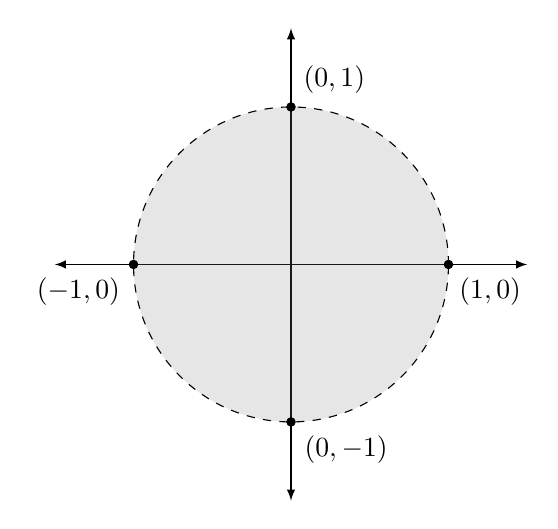
\begin{tikzpicture}
                \draw[latex-latex] (-3,0) -- (3,0);
                \draw[latex-latex] (0,-3) -- (0,3);

                \filldraw[dashed, fill=gray, fill opacity=0.2] (0,0) circle (2);

                \filldraw (-2,0) circle (1.5pt);
                \filldraw (0,2) circle (1.5pt);
                \filldraw (2,0) circle (1.5pt);
                \filldraw (0,-2) circle (1.5pt);

                \node at (-2.7,-0.35) {\( (-1, 0) \)};
                \node at (0.55, 2.35) {\( (0, 1) \)};
                \node at (2.53,-0.35) {\( (1, 0) \)};
                \node at (0.7,-2.35) {\( (0, -1) \)};
            \end{tikzpicture}
            \caption{\( V_1(0) \) with respect to \( d \)}
            \label{fig:2sub1}
        \end{subfigure}
        \begin{subfigure}{0.47\textwidth}
            \centering
            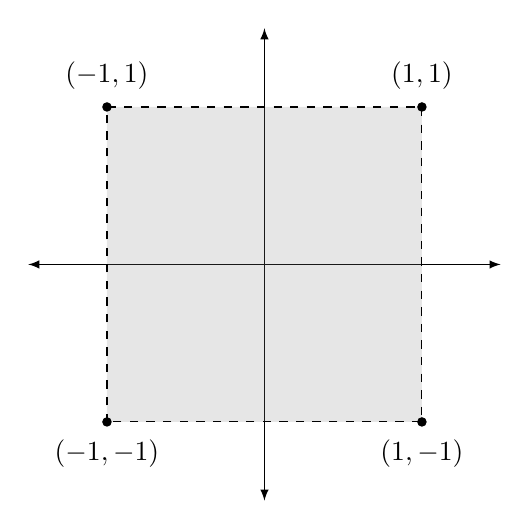
\begin{tikzpicture}
                \draw[latex-latex] (-3,0) -- (3,0);
                \draw[latex-latex] (0,-3) -- (0,3);

                \filldraw[dashed, fill=gray, fill opacity=0.2] (-2,-2) -- (-2,2) -- (2,2) -- (2,-2) -- (-2,-2);

                \filldraw (-2,-2) circle (1.5pt);
                \filldraw (-2,2) circle (1.5pt);
                \filldraw (2,2) circle (1.5pt);
                \filldraw (2,-2) circle (1.5pt);

                \node at (-2,-2.4) {\( (-1, -1) \)};
                \node at (-2,2.4) {\( (-1, 1) \)};
                \node at (2,2.4) {\( (1, 1) \)};
                \node at (2,-2.4) {\( (1, -1) \)};
            \end{tikzpicture}
            \caption{\( V_1(0) \) with respect to \( d' \)}
            \label{fig:2sub2}
        \end{subfigure}
        \caption{\( V_1(0) \) with respect to \( d \) and \( d' \)}
        \label{fig:2}
    \end{figure}
\end{solution}

\begin{exercise}
\label{ex:8}
    Let \( (X, d) \) be a metric space.
    \begin{enumerate}
        \item Verify that a typical \( \epsilon \)-neighborhood \( V_{\epsilon}(x) \) is an open set. Is the set
        \[
            C_{\epsilon}(x) = \{ y \in X : d(x, y) \leq \epsilon \}
        \]
        a closed set?

        \item Show that a set \( E \subseteq X \) is open if and only if its complement is closed.
    \end{enumerate}
\end{exercise}

\begin{solution}
    \begin{enumerate}
        \item Let \( \epsilon > 0 \) and \( x \in X \) be fixed. Given a \( y \in V_{\epsilon}(x) \), let \( \delta = \epsilon - d(x, y) > 0 \); we claim that \( V_{\delta}(y) \subseteq V_{\epsilon}(x) \). To see this, suppose that \( z \in V_{\delta}(y) \), so that
        \[
            d(z, y) < \delta = \epsilon - d(x, y) \quiff d(z, y) + d(x, y) < \epsilon.
        \]
        The triangle inequality now implies that
        \[
            d(z, x) \leq d(z, y) + d(x, y) < \epsilon.
        \]
        Thus \( z \in V_{\epsilon}(x) \) and it follows that \( V_{\delta}(y) \subseteq V_{\epsilon}(x) \); see \Cref{fig:3}, which shows the special case of \( \R^2 \) with the usual metric. As \( y \in V_{\epsilon}(x) \) was arbitrary, we may conclude that \( V_{\epsilon}(x) \) is an open set.

        \begin{figure}[H]
            \centering
            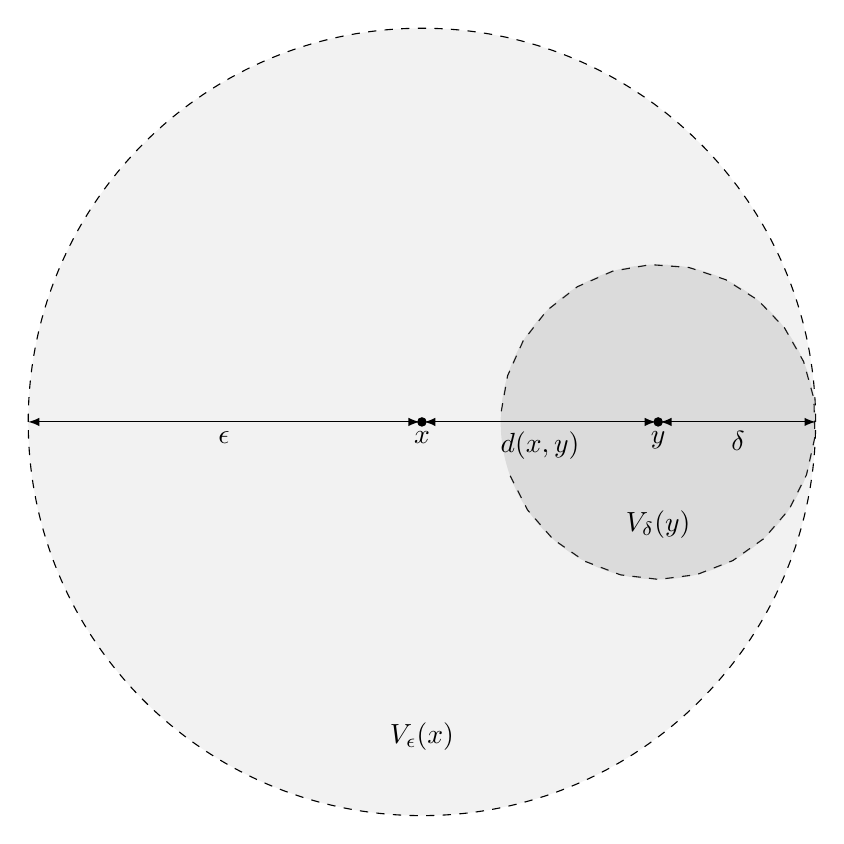
\begin{tikzpicture}
                \filldraw[dashed, fill=gray, fill opacity=0.1] (0,0) circle (5);
                \filldraw (0,0) circle (1.5pt) node[anchor=north] {\( x \)};
                \node at (0,-4) {\( V_{\epsilon}(x) \)};

                \draw[dashed,domain=-160:177] plot ({3 + 2*cos(\x)}, {2*sin(\x)});
                \fill[fill=gray, fill opacity=0.2] (3,0) circle (2);
                \filldraw (3,0) circle (1.5pt) node[anchor=north] {\( y \)};
                \node at (3,-1.3) {\( V_{\delta}(y) \)};

                \draw[latex-latex] (-5,0) -- (-0.03,0) node[anchor=north, pos=0.5] {\( \epsilon \)};
                \draw[latex-latex] (0.03,0) -- (2.97,0) node[anchor=north, pos=0.5] {\( d(x, y) \)};
                \draw[latex-latex] (3.03,0) -- (5,0) node[anchor=north, pos=0.5] {\( \delta \)};
            \end{tikzpicture}
            \caption{\( V_{\epsilon}(x) \) is open}
            \label{fig:3}
        \end{figure}

        Now we will show that, for \( \epsilon > 0 \) and \( x \in X \), the set \( C_{\epsilon}(x) \) is closed. To see this, let's prove the following:
        \[
            \text{if } y \in X \text{ is such that } d(x, y) > \epsilon \text{ then } y \text{ is not a limit point of } C_{\epsilon}(x).
        \]
        Let \( \delta = d(x, y) - \epsilon > 0 \) and suppose \( z \in V_{\delta}(y) \), so that
        \[
            d(z, y) < \delta = d(x, y) - \epsilon \quiff d(x, y) - d(z, y) > \epsilon.
        \]
        By the triangle inequality, we have
        \[
            d(x, y) \leq d(z, x) + d(z, y) \quimplies d(z, x) \geq d(x, y) - d(z, y) > \epsilon.
        \]
        Thus \( d(z, x) > \epsilon \), so that \( z \not\in C_{\epsilon}(x) \). We have now shown that there is a \( \delta > 0 \) such that \( V_{\delta}(y) \cap C_{\epsilon}(x) = \emptyset \); see \Cref{fig:4}, which shows the special case of \( \R^2 \) with the usual metric. It follows that \( y \) is not a limit point of \( C_{\epsilon}(x) \).

        \begin{figure}[H]
            \centering
            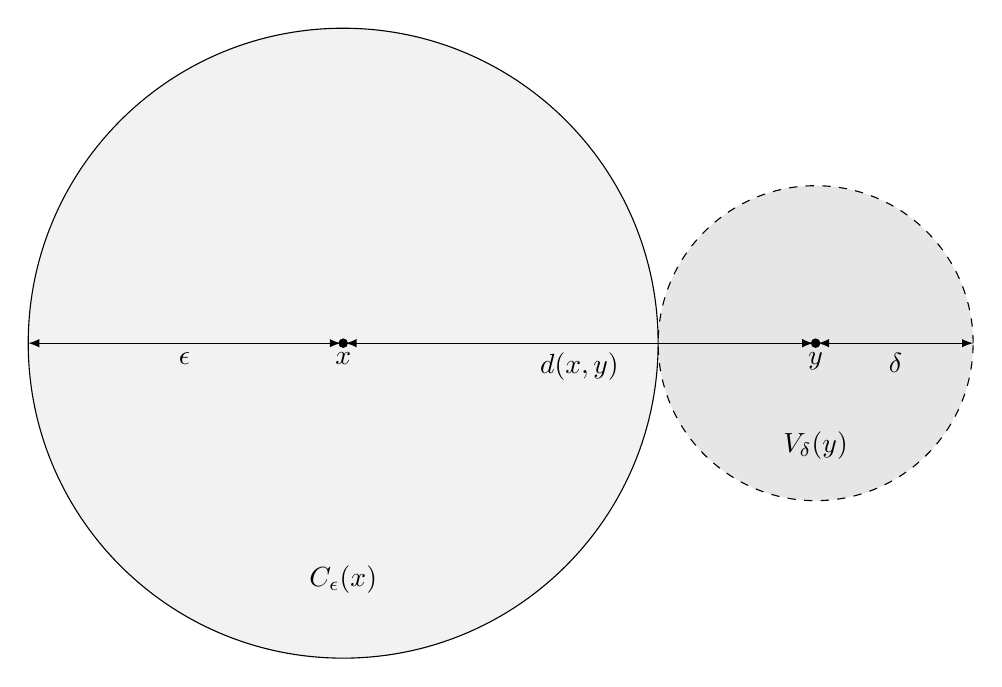
\begin{tikzpicture}
                \filldraw[fill=gray, fill opacity=0.1] (-2,0) circle (4);
                \filldraw (-2,0) circle (1.5pt) node[anchor=north] {\( x \)};
                \node at (-2,-3) {\( C_{\epsilon}(x) \)};

                \filldraw[dashed, fill=gray, fill opacity=0.2] (4,0) circle (2);
                \filldraw (4,0) circle (1.5pt) node[anchor=north] {\( y \)};
                \node at (4,-1.3) {\( V_{\delta}(y) \)};

                \draw[latex-latex] (-6,0) -- (-2.03,0) node[anchor=north, pos=0.5] {\( \epsilon \)};
                \draw[latex-latex] (-1.97,0) -- (3.97,0) node[anchor=north, pos=0.5] {\( d(x, y) \)};
                \draw[latex-latex] (4.03,0) -- (6,0) node[anchor=north, pos=0.5] {\( \delta \)};
            \end{tikzpicture}
            \caption{\( y \) is not a limit point of \( C_{\epsilon}(x) \)}
            \label{fig:4}
        \end{figure}

        The contrapositive of the statement just proven is:
        \[
            \text{if } y \in X \text{ is a limit point of } C_{\epsilon}(x) \text{ then } d(x, y) \leq \epsilon.
        \]
        In other words, if \( y \) is a limit point of \( C_{\epsilon}(x) \) then \( y \) belongs to \( C_{\epsilon}(x) \). We may conclude that \( C_{\epsilon}(x) \) is a closed set.

        \item Observe that
        \begin{align*}
            E \text{ is not open} &\iff (\exists x \in E)  (\forall \epsilon > 0) (V_{\epsilon}(x) \not\subseteq E) \\[2mm]
            &\iff (\exists x \in E) (\forall \epsilon > 0) \paren{ V_{\epsilon}(x) \cap \setcomp{E} \neq \emptyset } \\[2mm]
            &\iff (\exists x \in E) (\forall \epsilon > 0) \paren{ V_{\epsilon}(x) \cap \paren{ \setcomp{E} \setminus \{ x \} } \neq \emptyset } \\[2mm]
            &\iff (\exists x \in E) (x \text{ is a limit point of } \setcomp{E}) \\[2mm]
            &\iff \setcomp{E} \text{ does not contain all of its limit points} \\[2mm]
            &\iff \setcomp{E} \text{ is not closed}.
        \end{align*}
    \end{enumerate}
\end{solution}

\begin{exercise}
\label{ex:9}
    \begin{enumerate}
        \item Show that the set \( Y = \{ f \in C[0, 1] : \norm{f}_{\infty} \leq 1 \} \) is closed in \( C[0, 1] \).

        \item Is the set \( T = \{ f \in C[0, 1] : f(0) = 0 \} \) open, closed, or neither in \( C[0, 1] \)?
    \end{enumerate}
\end{exercise}

\begin{solution}
    \begin{enumerate}
        \item Using the notation of \Cref{ex:2} (a), observe that \( Y = C_1(0) \) (by 0 we mean the function which is identically zero on \( [0, 1] \)). Thus, by \Cref{ex:2} (a), \( Y \) is closed.

        \item \( T \) is not open. To see this, first observe that \( 0 \in T \). Now let \( \epsilon > 0 \) be given and define \( f_{\epsilon} \in C[0, 1] \) by \( f_{\epsilon}(x) = \tfrac{\epsilon}{2} \). Then
        \[
            d(f_{\epsilon}, 0) = \frac{\epsilon}{2} < \epsilon,
        \]
        so that \( f_{\epsilon} \in V_{\epsilon}(0) \). However, \( f_{\epsilon} \not\in T \) and so \( V_{\epsilon}(0) \not\subseteq T \). As \( \epsilon > 0 \) was arbitrary, we may conclude that \( T \) is not open.

        \( T \) is closed. To see this, suppose that \( g \in C[0, 1] \) is a limit point of \( T \) and let \( \epsilon > 0 \) be given. There exists some \( f \in V_{\epsilon}(g) \cap T \) such that \( f \neq g \) and it follows that
        \[
            \abs{g(0)} = \abs{g(0) - f(0)} \leq d(g, f) < \epsilon.
        \]
        As \( \epsilon > 0 \) was arbitrary, we see that \( g(0) = 0 \), so that \( g \in T \). Thus \( T \) contains its limit points, i.e.\ \( T \) is closed.
    \end{enumerate}
\end{solution}

\begin{exercise}
\label{ex:10}
    \begin{enumerate}
        \item Supply a definition for \textit{bounded} subsets of a metric space \( (X, d) \).

        \item Show that if \( K \) is a compact subset of the metric space \( (X, d) \), then \( K \) is closed and bounded.

        \item Show that \( Y \subseteq C[0, 1] \) from \Cref{ex:9} (a) is closed and bounded but not compact.
    \end{enumerate}
\end{exercise}

\begin{solution}
    \begin{enumerate}
        \item A subset \( E \subseteq X \) is bounded if there exists some \( y \in X \) and \( M > 0 \) such that \( d(x, y) \leq M \) for all \( x \in E \), i.e.\ \( E \subseteq C_M(y) \).

        \item We will prove the contrapositive statement. First, suppose that \( K \) is not closed. Then there exists some \( y \not\in K \) such that \( y \) is a limit point of \( K \). Thus, for each \( n \in \N \), there exists some \( x_n \in V_{n^{-1}}(y) \cap K \), i.e.\ there is some \( x_n \in K \) such that \( d(x_n, y) < \tfrac{1}{n} \). Given this, it is clear that \( (x_n) \) converges to \( y \). It is straightforward to prove the analogous statement to Theorem 2.5.2 for metric spaces:
        
        \begin{tcolorbox}[colback=blue!5!white]
            Let \( (X, d) \) be a metric space and suppose that \( (x_n) \) is a sequence in \( X \) which converges to some \( x \in X \). If \( \paren{ x_{n_k} } \) is a subsequence of \( (x_n) \), then \( \paren{ x_{n_k} } \) also converges to \( x \).
            \tcblower
            \textit{Proof.} Let \( \epsilon > 0 \) be given. As \( \lim_{n \to \infty} x_n = x \), there is an \( N \in \N \) such that \( d(x_n, x) < \epsilon \) for all \( n \geq N \). Because \( \paren{ x_{n_k} } \) is a subsequence of \( (x_n) \), there must exist some \( K \in \N \) such that \( n_k \geq N \) for all \( k \geq K \); for such \( k \), we then have \( d \paren{ x_{n_k}, x } < \epsilon \). It follows that \( \lim_{k \to \infty} x_{n_k} = x \). \qed
        \end{tcolorbox}
        
        Hence any subsequence of \( (x_n) \) must also converge to \( y \), which does not belong to \( K \); it follows that \( K \) is not compact.

        Next, suppose that \( K \) is not bounded and pick some \( x_1 \in K \). Because \( K \) is not bounded, it must be the case that \( K \) is not contained in \( C_1(x_1) \), so that there exists some \( x_2 \in K \) satisfying \( d(x_1, x_2) > 1 \). Similarly, it must be the case that \( K \) is not contained in \( C_1(x_1) \cup C_1(x_2) \), so that there exists some \( x_3 \in K \) satisfying \( d(x_1, x_3) > 1 \) and \( d(x_2, x_3) > 1 \). If we continue in this manner, we obtain a sequence \( (x_n) \) in \( K \) such that \( d(x_m, x_n) > 1 \) for all \( n > m \). Suppose that \( \paren{ x_{n_k} } \) is a subsequence of \( (x_n) \) and observe that for any \( K \in \N \) we have \( d \paren{ x_{n_K}, x_{n_{K+1}} } > 1 \). It follows that \( \paren{ x_{n_k} } \) is not Cauchy and hence not convergent (\Cref{ex:4}). As \( \paren{ x_{n_k} } \) was an arbitrary subsequence, we see that \( K \) is not compact.

        \item We showed in \Cref{ex:9} (a) that \( Y \) is closed, and it is clearly bounded. To see that \( Y \) is not compact, consider the sequence of functions \( (f_n) \) given by \( f_n(x) = x^n \), each of which is continuous on \( [0, 1] \), satisfies \( \norm{f_n}_{\infty} = 1 \), and hence belongs to \( Y \). We will argue by contradiction to show that \( (f_n) \) has no convergent subsequence. If \( \paren{ f_{n_k} } \) is a subsequence converging to some \( f \in C[0, 1] \), then in particular \( f \) is the pointwise limit of \( \paren{ f_{n_k} } \) on \( [0, 1] \). However, we can see directly that the pointwise limit of \( \paren{ f_{n_k} } \) is the function
        \[
            x \mapsto \begin{cases}
                0 & \text{if } 0 \leq x < 1, \\
                1 & \text{if } x = 1.
            \end{cases}
        \]
        Since limits are unique (Theorem 2.2.7), it must be the case that \( f \) is given by the function above, which is not continuous at \( x = 1 \), contradicting that \( f \in C[0, 1] \).
    \end{enumerate}
\end{solution}

\begin{exercise}
\label{ex:11}
    \begin{enumerate}
        \item Show that \( E \) is closed if and only if \( \overline{E} = E \). Show that \( E \) is open if and only if \( \interior{E} = E \).

        \item Show that \( \setcomp{\overline{E}} = \interior{\paren{\setcomp{E}}} \), and similarly that \( \setcomp{\paren{\interior{E}}} = \overline{\setcomp{E}} \).
    \end{enumerate}
\end{exercise}

\begin{solution}
    \begin{enumerate}
        \item See \href{https://lew98.github.io/Mathematics/UA_Section_3_2_Exercises.pdf}{Exercise 3.2.14} (a).

        \item See \href{https://lew98.github.io/Mathematics/UA_Section_3_2_Exercises.pdf}{Exercise 3.2.14} (b).
    \end{enumerate}
\end{solution}

\begin{exercise}
\label{ex:12}
    \begin{enumerate}
        \item Show
        \[
            \overline{V_{\epsilon}(x)} \subseteq \{ y \in X : d(x, y) \leq \epsilon \},
        \]
        is an arbitrary metric space \( (X, d) \).

        \item To keep things from sounding too familiar, find an example of a specific metric space where
        \[
            \overline{V_{\epsilon}(x)} \neq \{ y \in X : d(x, y) \leq \epsilon \}.
        \]
    \end{enumerate}
\end{exercise}

\begin{solution}
    \begin{enumerate}
        \item Using the notation from \Cref{ex:8}, note that \( \{ y \in X : d(x, y) \leq \epsilon \} = C_{\epsilon}(x) \). Clearly \( V_{\epsilon}(x) \subseteq C_{\epsilon}(x) \) and thus if \( y \) is a limit point of \( V_{\epsilon}(x) \) then \( y \) is also a limit point of \( C_{\epsilon}(x) \). As we showed in \Cref{ex:8}, \( C_{\epsilon}(x) \) is closed and hence \( y \in C_{\epsilon}(x) \). We may conclude that \( \overline{V_{\epsilon}(x)} \subseteq C_{\epsilon}(x) \).

        \item Consider the metric space \( (\R, \rho) \), where \( \rho \) is the discrete metric. Then
        \[
            \overline{V_1(0)} = \overline{\{ 0 \}} = \overline{C_{1/2}(0)} = C_{1/2}(0) = \{ 0 \} \neq \R = C_1(0).
        \]
    \end{enumerate}
\end{solution}

\begin{exercise}
\label{ex:13}
    If \( E \) is a subset of a metric space \( (X, d) \), show that \( E \) is nowhere-dense in \( X \) if and only if \( \setcomp{\overline{E}} \) is dense in \( X \).
\end{exercise}

\begin{solution}
    For the purposes of this exercise, let us denote by \( \kappa E \) the closure of \( E \), by \( \iota E \) the interior of \( E \), and by \( c E \) the complement of \( E \). Observe that:
    \begin{align*}
        c \kappa E \text{ is dense in } X &\iff \kappa c \kappa E = X \\[2mm]
        &\iff c \kappa c \kappa E = \emptyset \\[2mm]
        &\iff \iota c c \kappa E = \emptyset \tag{\Cref{ex:11} (b)} \\[2mm]
        &\iff \iota \kappa E = \emptyset \\[2mm]
        &\iff E \text{ is nowhere-dense in } X.
    \end{align*}
\end{solution}

\begin{exercise}
\label{ex:14}
    \begin{enumerate}
        \item Give the details for why we know there exists a point \( x_2 \in V_{\epsilon_1}(x_1) \cap O_2 \) and an \( \epsilon_2 > 0 \) satisfying \( \epsilon_2 < \epsilon_1/2 \) with \( V_{\epsilon_2}(x_2) \) contained in \( O_2 \) and
        \[
            \overline{V_{\epsilon_2}(x_2)} \subseteq V_{\epsilon_1}(x_1).
        \]
        
        \item Proceed along this line and use the completeness of \( (X, d) \) to produce a single point \( x \in O_n \) for every \( n \in \N \).
    \end{enumerate}
\end{exercise}

\begin{solution}
    \begin{enumerate}
        \item Note that \( x_1 \) must be a limit point of \( O_2 \) as \( O_2 \) is dense in \( X \) and thus there exists some \( x_2 \in V_{\epsilon_1}(x_1) \cap O_2 \). Since \( O_2 \) is open, there exists some \( \delta > 0 \) such that \( V_{\delta}(x_2) \subseteq O_2 \). If we let
        \[
            \epsilon_2 = \min \set{ \delta, \frac{\epsilon_1}{4}, r := \frac{\epsilon_1 - d(x_1, x_2)}{2} },
        \]
        then:
        \begin{itemize}
            \item \( V_{\epsilon_2}(x_2) \subseteq V_{\delta}(x_2) \subseteq O_2 \);

            \item \( \epsilon_2 < \tfrac{\epsilon_1}{2} \);

            \item \( \overline{V_{\epsilon_2}(x_2)} \subseteq \overline{V_r(x_2)} \subseteq C_r(x_2) \subseteq V_{\epsilon_1}(x_1) \), where we have used \Cref{ex:12} (a) for the second inclusion.
        \end{itemize}

        \item By continuing this process, we obtain a sequence \( (x_n) \) of points in \( X \) and a sequence \( (\epsilon_n) \) of real numbers such that:
        \begin{enumerate}[label=(\roman*)]
            \item \( \epsilon_n < \tfrac{\epsilon_1}{2^{n-1}} \) for each \( n \geq 2 \);
            
            \item \( V_{\epsilon_n}(x_n) \subseteq O_n \) for each \( n \in \N \);

            \item the following chain of inclusions holds:
            \begin{multline*}
                \cdots \subseteq V_{\epsilon_n}(x_n) \subseteq \overline{V_{\epsilon_n}(x_n)} \subseteq V_{\epsilon_{n-1}}(x_{n-1}) \subseteq \overline{V_{\epsilon_{n-1}}(x_{n-1})} \\[2mm]
                \subseteq \cdots \subseteq V_{\epsilon_2}(x_2) \subseteq \overline{V_{\epsilon_2}(x_2)} \subseteq V_{\epsilon_1}(x_1) \subseteq \overline{V_{\epsilon_1}(x_1)}.
            \end{multline*}
        \end{enumerate}
        By (i), for any \( \epsilon > 0 \) we can choose an \( N \geq 2 \) such that \( 2 \epsilon_N < \epsilon \). Suppose \( n \geq m \geq N \). By (iii) we have \( x_m, x_n \in V_{\epsilon_N}(x_N) \) and thus
        \[
            d(x_m, x_n) \leq d(x_m, x_N) + d(x_n, x_N) < 2 \epsilon_N < \epsilon.
        \]
        It follows that \( (x_n) \) is a Cauchy sequence. By assumption the metric space \( (X, d) \) is complete and so there exists some \( x_0 \) such that \( \lim x_n = x_0 \).

        For any \( m \in \N \), (iii) implies that the sequence \( (x_n) \) is eventually contained inside the set \( \overline{V_{\epsilon_{m+1}}(x_{m+1})} \); it follows that \( x_0 \) is a limit point of \( \overline{V_{\epsilon_{m+1}}(x_{m+1})} \). Since this set is closed, we have by (ii) and (iii):
        \[
            x_0 \in \overline{V_{\epsilon_{m+1}}(x_{m+1})} \subseteq V_{\epsilon_m}(x_m) \subseteq O_m.
        \]
        Thus \( x_0 \in \bigcap_{m=1}^{\infty} O_m \).
    \end{enumerate}
\end{solution}

\begin{exercise}
\label{ex:15}
    Complete the proof of the theorem.
\end{exercise}

\begin{solution}
    Let \( (X, d) \) be a complete metric space and suppose \( \{ E_n : n \in \N \} \) is a countable collection of nowhere-dense sets. Notice that each \( \setcomp{\overline{E_n}} \) is open (\Cref{ex:8} (b)) and dense (\Cref{ex:13}); it follows from Theorem 8.2.10 that \( \bigcap_{n=1}^{\infty} \setcomp{\overline{E_n}} \neq \emptyset \). Now observe that
    \[
        E_n \subseteq \overline{E_n} \text{ for each } n \in \N \quimplies \setcomp{\overline{E_n}} \subseteq \setcomp{E_n} \text{ for each } n \in \N \quimplies \bigcap_{n=1}^{\infty} \setcomp{\overline{E_n}} \subseteq \bigcap_{n=1}^{\infty} \setcomp{E_n}.
    \]
    Thus \( \bigcap_{n=1}^{\infty} \setcomp{E_n} \neq \emptyset \), which implies that
    \[
        X \neq \setcomp{\paren{ \bigcap_{n=1}^{\infty} \setcomp{E_n} }} = \bigcup_{n=1}^{\infty} E_n.
    \]
\end{solution}

\begin{exercise}
\label{ex:16}
    Show that if \( f \in C[0, 1] \) is differentiable at a point \( x \in [0, 1] \), then \( f \in A_{m,n} \) for some pair \( m, n \in \N \).
\end{exercise}

\begin{solution}
    By assumption we have
    \[
        f'(x) = \lim_{t \to x} \frac{f(x) - f(t)}{x - t}
    \]
    and thus there exists a \( \delta > 0 \) such that
    \[
        0 < \abs{x - t} < \delta \quimplies \abs{\frac{f(x) - f(t)}{x - t} - f'(x)} < 1.
    \]
    Let \( m \in \N \) be such that \( \tfrac{1}{m} < \delta \) and let \( n \in \N \) be such that \( 1 + \abs{f'(x)} \leq n \). Then:
    \[
        0 < \abs{x - t} < \frac{1}{m} < \delta \implies \abs{\frac{f(x) - f(t)}{x - t}} \leq \abs{\frac{f(x) - f(t)}{x - t} - f'(x)} + \abs{f'(x)} < 1 + \abs{f'(x)} \leq n.
    \]
    Thus \( f \in A_{m,n} \).
\end{solution}

\begin{exercise}
\label{ex:17}
    \begin{enumerate}
        \item The sequence \( (x_k) \) does not necessarily converge, but explain why there exists a subsequence \( \paren{ x_{k_l} } \) that is convergent. Let \( x = \lim \paren{ x_{k_l} } \).

        \item Prove that \( f_{k_l} \paren{ x_{k_l} } \to f(x) \).

        \item Now finish the proof that \( A_{m,n} \) is closed.
    \end{enumerate}
\end{exercise}

\begin{solution}
    \begin{enumerate}
        \item The sequence \( (x_n) \) is contained in the interval \( [0, 1] \) and thus by the Bolzano-Weierstrass Theorem (Theorem 2.5.5) there exists a convergent subsequence \( \paren{ x_{k_l} } \).

        \item Let \( \epsilon > 0 \) be given. As \( f_k \to f \) in \( C[0, 1] \), there is an \( L_1 \in \N \) such that
        \[
            l \geq L_1 \quimplies d \paren{ f_{k_l}, f } < \frac{\epsilon}{2}.
        \]
        The continuity of \( f \) at \( x \) implies that \( \lim_{l \to \infty} f \paren{ x_{k_l} } = f(x) \) and thus there is an \( L_2 \in \N \) such that
        \[
            l \geq L_2 \quimplies \abs{ f \paren{ x_{k_l} } - f(x) } < \frac{\epsilon}{2}.
        \]
        Now observe that for \( l \geq \max \{ L_1, L_2 \} \) we have
        \[
            \abs{ f_{k_l} \paren{ x_{k_l} } - f(x)} \leq \abs{ f_{k_l} \paren{ x_{k_l} } - f \paren{ x_{k_l} }} + \abs{f \paren{ x_{k_l} } - f(x)} \leq d \paren{ f_{k_l}, f } + \frac{\epsilon}{2} < \epsilon.
        \]
        It follows that \( f_{k_l} \paren{ x_{k_l} } \to f(x) \).

        \item Suppose \( t \) is such that \( 0 < \abs{x - t} < \tfrac{1}{m} \). Because \( x_{k_l} \to x \), there is an \( L \in \N \) such that
        \[
            l \geq L \quimplies \abs{x - x_{k_l}} < \frac{1}{m} - \abs{x - t} \quimplies \abs{x_{k_l} - t} \leq \abs{x - x_{k_l}} + \abs{x - t} < \frac{1}{m}.
        \]
        This implies that
        \[
            \abs{ \frac{f_{k_l} \paren{ x_{k_l} } - f_{k_l}(t)}{x_{k_l} - t} } \leq n \quad \text{ for all } l \geq L.
        \]
        Taking the limit as \( l \to \infty \) on both sides of this inequality and using part (b), we see that
        \[
            \abs{ \frac{f(x) - f(t)}{x - t} } \leq n
        \]
        and hence \( f \in A_{m,n} \). We may conclude that \( A_{m,n} \) contains its limit points and hence is closed.
    \end{enumerate}
\end{solution}

\begin{exercise}
\label{ex:18}
    A continuous function is called \textit{polygonal} if its graph consists of a finite number of line segments.
    \begin{enumerate}
        \item Show that there exists a polygonal function \( p \in C[0, 1] \) satisfying \( \norm{f - p}_{\infty} < \epsilon/2 \).

        \item Show that if \( h \) is any function in \( C[0, 1] \) that is bounded by 1, then the function
        \[
            g(x) = p(x) + \frac{\epsilon}{2} h(x)
        \]
        satisfies \( g \in V_{\epsilon}(f) \).

        \item Construct a polygonal function \( h(x) \) in \( C[0, 1] \) that is bounded by 1 and leads to the conclusion \( g \not\in A_{m,n} \), where \( g \) is defined as in (b). Explain how this completes the argument for Theorem 8.2.12.
    \end{enumerate}
\end{exercise}

\begin{solution}
    \begin{enumerate}
        \item This follows from Theorem 6.7.3, which we proved in \href{https://lew98.github.io/Mathematics/UA_Section_6_7_Exercises.pdf}{Exercise 6.7.2}.

        \item Observe that
        \[
            \norm{f - g}_{\infty} = \norm{ f - p - \tfrac{\epsilon}{2} h }_{\infty} \leq \norm{f - p}_{\infty} + \norm{\tfrac{\epsilon}{2}h}_{\infty} < \epsilon.
        \]

        \item Because \( p \) is polygonal, there are points \( 0 = x_0 < \cdots < x_N = 1 \) such that \( p \) is a line segment on \( [x_{k-1}, x_k] \); for each \( 1 \leq k \leq N \), let \( M_k \) be the slope of this line segment. Define \( M = \max \{ \abs{M_1}, \ldots, \abs{M_N} \} \) and let \( h \in C[0, 1] \) be the sawtooth function whose slope has absolute value \( \tfrac{2}{\epsilon} (M + n + 1) \) as in \Cref{fig:5}.
        
        \begin{figure}[H]
            \centering
            \begin{tikzpicture}
                \draw[-latex] (0,0) -- (8,0);
                \draw[-latex] (0,0) -- (0,8);
                \filldraw (0,0) circle (1.5pt) node[anchor=north] {\( 0 \)};
                \filldraw (7,0) circle (1.5pt) node[anchor=north] {\( 1 \)};
                \filldraw (0,7) circle (1.5pt) node[anchor=east] {\( 1 \)};

                \draw (0,0) -- (2,7) -- (4,0) -- (6,7) -- (7,3.5);

                \node at (4,7.7) {slope = \( \tfrac{2}{\epsilon} (M + n + 1) \)};
                \draw[-latex] (4,7.3) -- (5.4,5.6);
            \end{tikzpicture}
            \caption{\( h \) on \( [0, 1] \)}
            \label{fig:5}
        \end{figure}
        
        For any given \( x \in [0, 1] \), we have \( x \in [x_{k-1}, x_k] \) for some \( 1 \leq k \leq N \). Note that we can always choose some \( t \in [0, 1] \) such that:
        \begin{itemize}
            \item \( 0 < \abs{x - t} < \tfrac{1}{m} \);

            \item \( t \in [x_{k-1}, x_k] \), so that \( x \) and \( t \) belong to the same line segment of \( p \);

            \item \( x \) and \( t \) belong to the same line segment of \( h \).
        \end{itemize}
        There are two cases. If \( x \) and \( t \) belong to a line segment of \( h \) which has slope \( \tfrac{2}{\epsilon} (M + n + 1) \), then
        \begin{multline*}
            \abs{ \frac{g(x) - g(t)}{x - t} } = \abs{ \frac{p(x) - p(t)}{x - t} + \frac{\epsilon}{2} \frac{h(x) - h(t)}{x - t} } \\[2mm]
            = \abs{M_k + M + n + 1} = M_k + M + n + 1 \geq n + 1 > n.
        \end{multline*}
        Similarly, if \( x \) and \( t \) belong to a line segment of \( h \) which has slope \( -\tfrac{2}{\epsilon} (M + n + 1) \), then
        \begin{multline*}
            \abs{ \frac{g(x) - g(t)}{x - t} } = \abs{ \frac{p(x) - p(t)}{x - t} + \frac{\epsilon}{2} \frac{h(x) - h(t)}{x - t} } \\[2mm]
            = \abs{M_k - M - n - 1} = n + 1 + M - M_k \geq n + 1 > n.
        \end{multline*}
        To summarize: for any \( x \in [0, 1] \) there exists a \( t \in [0, 1] \) such that \( 0 < \abs{x - t} < \tfrac{1}{m} \) and
        \[
            \abs{ \frac{g(x) - g(t)}{x - t} } > n;
        \]
        it follows that \( g \not\in A_{m,n} \).

        We have now shown that any \( \epsilon \)-neighbourhood of \( f \) contains some function \( g \) which does not belong to \( A_{m,n} \). As \( f \) was arbitrary, this implies that each \( A_{m,n} \) has empty interior. We showed in \Cref{ex:17} that each \( A_{m,n} \) was a closed set and thus each \( A_{m,n} \) is nowhere-dense in \( C[0, 1] \). It follows that the countable union
        \[
            \bigcup_{m=1}^{\infty} \bigcup_{n=1}^{\infty} A_{m,n}
        \]
        is a set of first category. We showed in \Cref{ex:16} that this union contains \( D \). Now, any subset of a set of first category is again a set of first category:

        \begin{tcolorbox}
            Let \( (X, d) \) be a metric space and suppose \( A \subseteq X \) is a set of first category, i.e.\ there is a countable collection \( \{ E_n : n \in \N \} \) of nowhere-dense sets such that \( A = \bigcup_{n=1}^{\infty} E_n \). If \( B \) is a subset of \( A \), then \( B \) is also a set of first category.
            \tcblower
            \textit{Proof.} For each \( n \in \N \), note that
            \[
                B \cap E_n \subseteq E_n \implies \overline{B \cap E_n} \subseteq \overline{E_n} \implies \interior{\paren{\overline{B \cap E_n}}} \subseteq \interior{\paren{\overline{E_n}}} = \emptyset.
            \]
            Thus \( \interior{\paren{\overline{B \cap E_n}}} = \emptyset \), so that each \( B \cap E_n \) is nowhere-dense in \( X \). Now observe that
            \[
                B = B \cap A = B \cap \bigcup_{n=1}^{\infty} E_n = \bigcup_{n=1}^{\infty} \paren{B \cap E_n}.
            \]
            This shows that \( B \) can be expressed as a countable union of nowhere-dense sets; it follows that \( B \) is a set of first category. \qed
        \end{tcolorbox}

        We may conclude that \( D \) is a set of first category.
    \end{enumerate}
\end{solution}

\noindent \hrulefill

\noindent \hypertarget{ua}{\textcolor{blue}{[UA]} Abbott, S. (2015) \textit{Understanding Analysis.} 2\ts{nd} edition.}

\end{document}